% !TeX spellcheck = en_US
\section{Traditional Feature-Based \ac{ser}}


\subsection{Feature Extraction}

Feature extraction is an essential component in audio analysis tasks, as it allows the transformation of raw audio data into a set of informative features that can capture key characteristics of the signal.

In this regard, the widely-used Librosa toolkit was employed to extract various audio features, from the audio files of the \ac{iemo} dataset, which were subsequently processed using statistical metrics. The extracted features and associated metrics are summarized in Table \ref{table:extractedFeat}, having in total, extracted 327 features.

\begin{table}[h]
	\centering
	\caption{Extracted Audio Features and Statistical Functions Applied to Them}
	\label{table:extractedFeat}
	
	\begin{tabular}{@{}cc@{}}
		\toprule
		Audio Features & Statistical Functions \\
		\midrule
		&  \multirow{10}{*}{\begin{tabular}{@{}c@{}}Minimum\\Mean\\Maximum\\Median\\25th percentile\\75th percentile\\Spikes\footnotemark[1]\\Variance \\Standard Deviation\\Sum\\Kurtosis\footnotemark[2]\\Skew\footnotemark[2]\end{tabular}} \\
		\acp{mfccs} 1 - 21 & \\
		Mel Spectrogram & \\
		Root-Mean-Square & \\
		Chromagram & \\
		Spectral Centroid & \\
		Spectral Contrast & \\
		Spectral Bandwith & \\
		Roll-Off Frequency & \\
		Tonnetz & \\
		Zero-Crossing Rate & \\
		& \\
		\bottomrule
		\multicolumn{2}{l}{\footnotemark[1]\footnotesize{Custom function detailed on the Feature Selection section.}} \\
		\multicolumn{2}{l}{\footnotemark[2]\footnotesize{Only for the \acp{mfccs}.}} \\
	\end{tabular}
\end{table}

\subsection{Feature Analysis}

One important task following feature extraction is to analyze and interpret the extracted data to gain a deeper understanding of the audio signals and the features that describe them.

\subsubsection{Audio Signal Study}

In this process, we visually analyzed and interpreted the features' data by graphically representing each feature from an audio segment. The figures in Section \ref{sec:App:1} of the appendix demonstrate some of the graphics we used to visualize the data.

\subsubsection{Spikes Metric}

Initially, wave plots were observed, and we noted consistency in the number of high values. For this reason, we created a custom metric that calculates those high values, which we called "spikes", from the features' data.

In Figure \ref{fig:zcrSpikes}, it is possible to visualize the zero crossing rates' wave plots in different emotions. The horizontal line represents the threshold that we considered, any value above was considered to be a spike, which is annotated with red dots in the graphic. The threshold used was manually tested and obtained decent consistency of the number of spikes, within an emotion, by using the mean value of the feature plus 2\% of the standard deviation. To account for different-length audio signals, it was also divided the number of spikes to the total length of the data, as the Code Snippet \ref{spikes:code} demonstrates. Consequently, this metric was also tested and applied to every other audio feature.

\begin{listing}[H]
	\begin{minted}{python}
def spikes(data):
	num_spikes = 0
	mean = np.mean(data)
	std = np.std(data)
	
	threshold = mean + np.abs(std) * 2 / 100
	for value in data:
		if value >= threshold:
			num_spikes += 1

	return num_spikes / len(data)
	\end{minted}
	\caption{Python code for calculating the spikes metric.}
	\label{spikes:code}
\end{listing}

\begin{figure}[H]
	\centering
	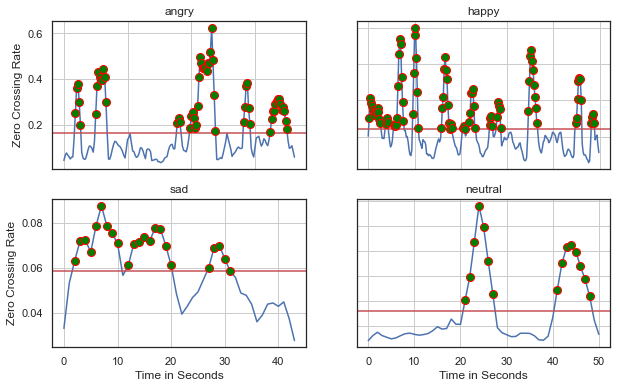
\includegraphics[width=.7\textwidth]{figs/4_1_traditional/zcr_waveplot_spikes.png}
	\caption{Zero crossing rate wave plot annotated with spikes.}
	\label{fig:zcrSpikes}
\end{figure}


\subsubsection{Bar Plots}

Furthermore, bar plots were useful for viewing the overall extracted features' data plainly and quickly, and to understand the numeric values of each feature and metric used on it.

For example, figure \ref{fig:melBarPlot} shows clear differences in the mean values for some metrics used on the Mel Spectrogram.

\begin{figure}[H]
	\centering
	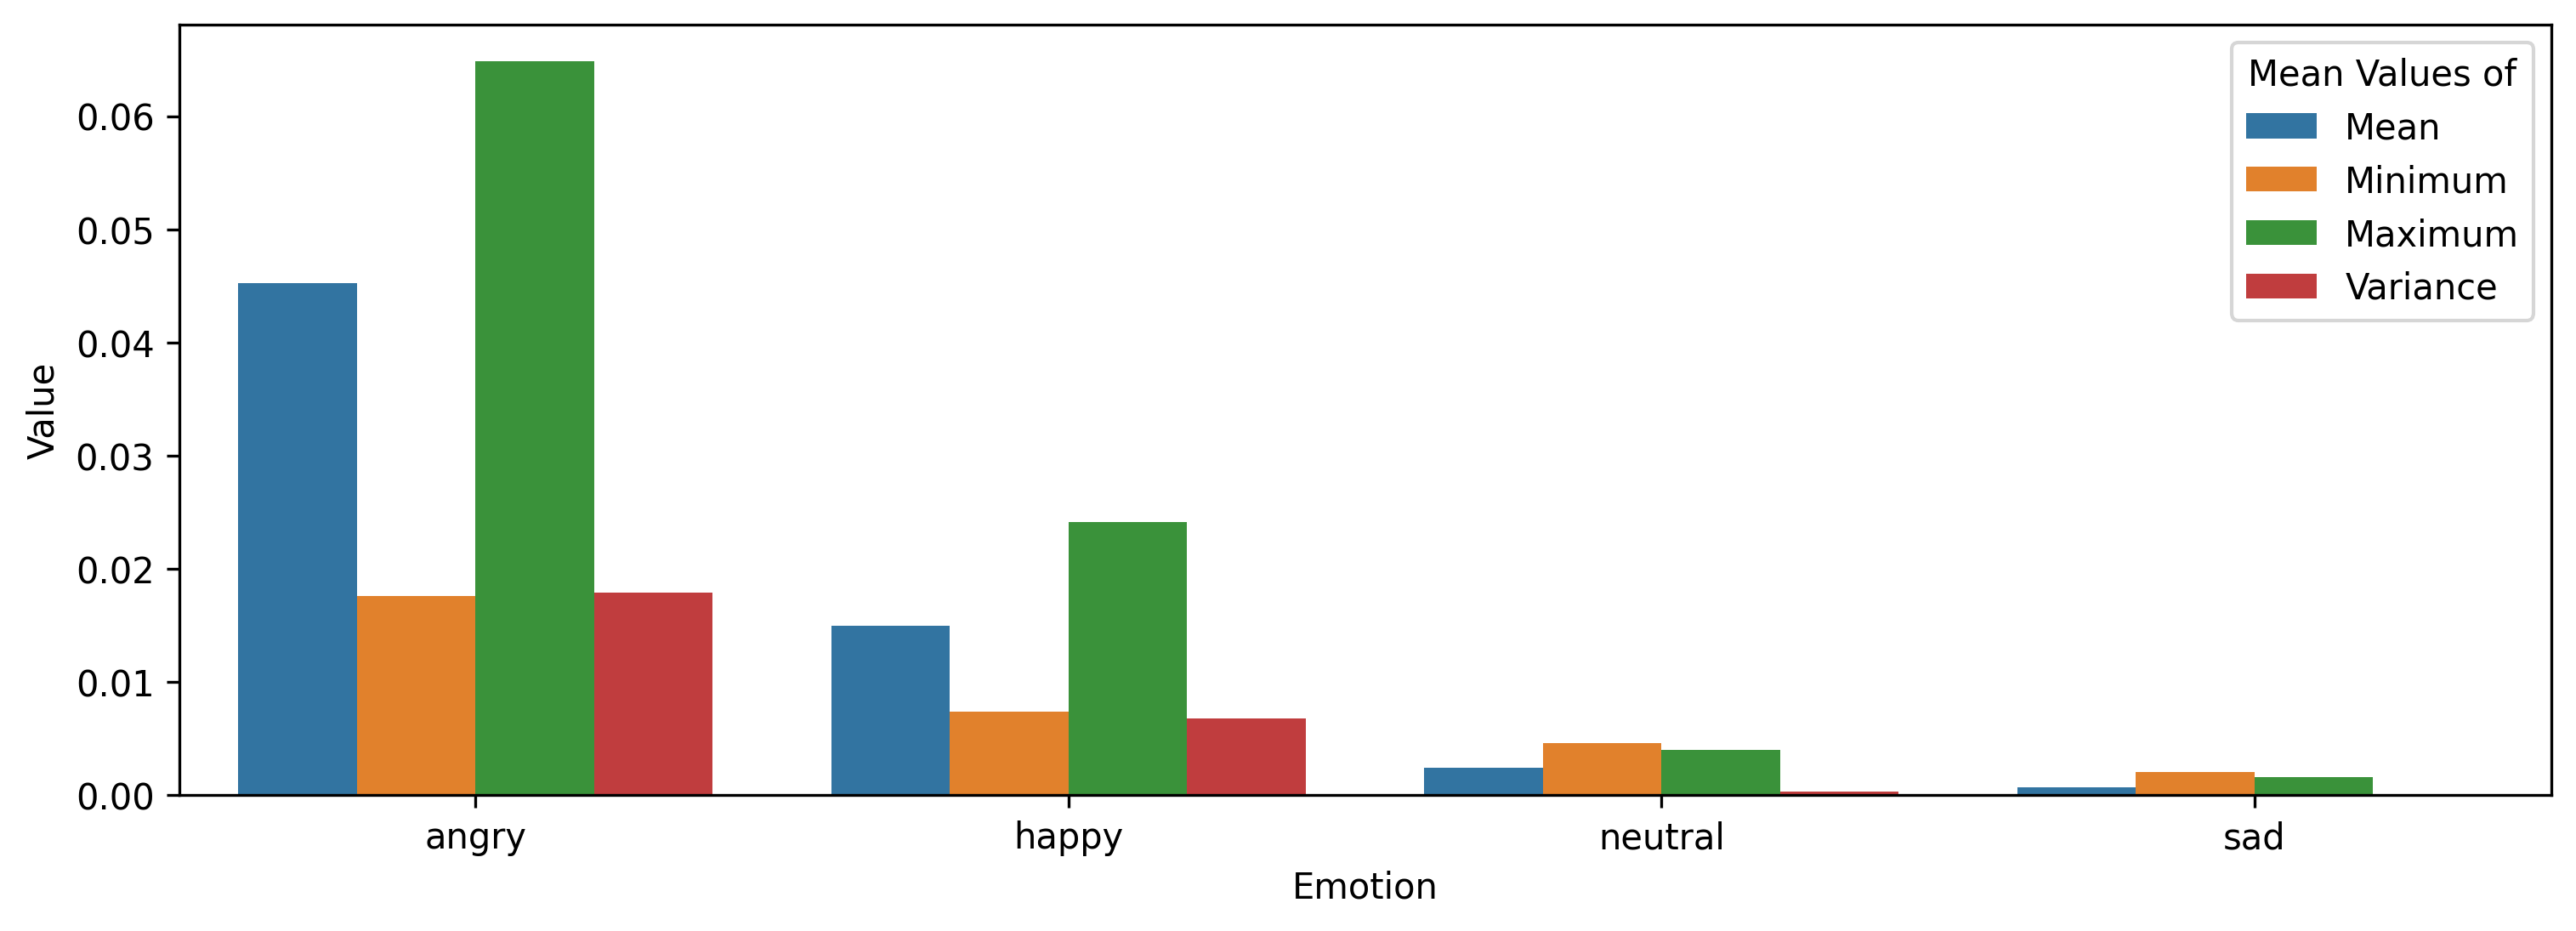
\includegraphics[width=\textwidth]{figs/4_1_traditional/meanFeatBarPlot.png}
	\caption{Bar plots mean for metrics used on the mel-scaled spectrogram feature}
	\label{fig:melBarPlot}
\end{figure}


\subsubsection{Wave Plots with Surrounding Areas}

During the feature study process, it was observed the wave plots of some features surrounded by a small area above and below the original wave (defined through a selected threshold). This was done to corroborate how well the feature describes different emotions. A high degree of overlap between surrounding areas of a feature on a given emotion for different subjects could indicate that the feature is relevant for representing that emotion.

Figure \ref{fig:zcrAreaOnly1} is an excerpt of the figure \ref{fig:zcrArea} in the appendix, and it demonstrates an example of this analysis for the zero crossing rate with 5 different subjects on the same sentence for the anger emotions.

From this graphic, it was observed that there is a sufficient amount of overlap between the surrounding areas for each emotion to conclude that the feature has some utility for describing each emotion. However, due to the different lengths of each audio segment, it is ambitious to guarantee this conclusion.

\begin{figure}[H]
	\centering
	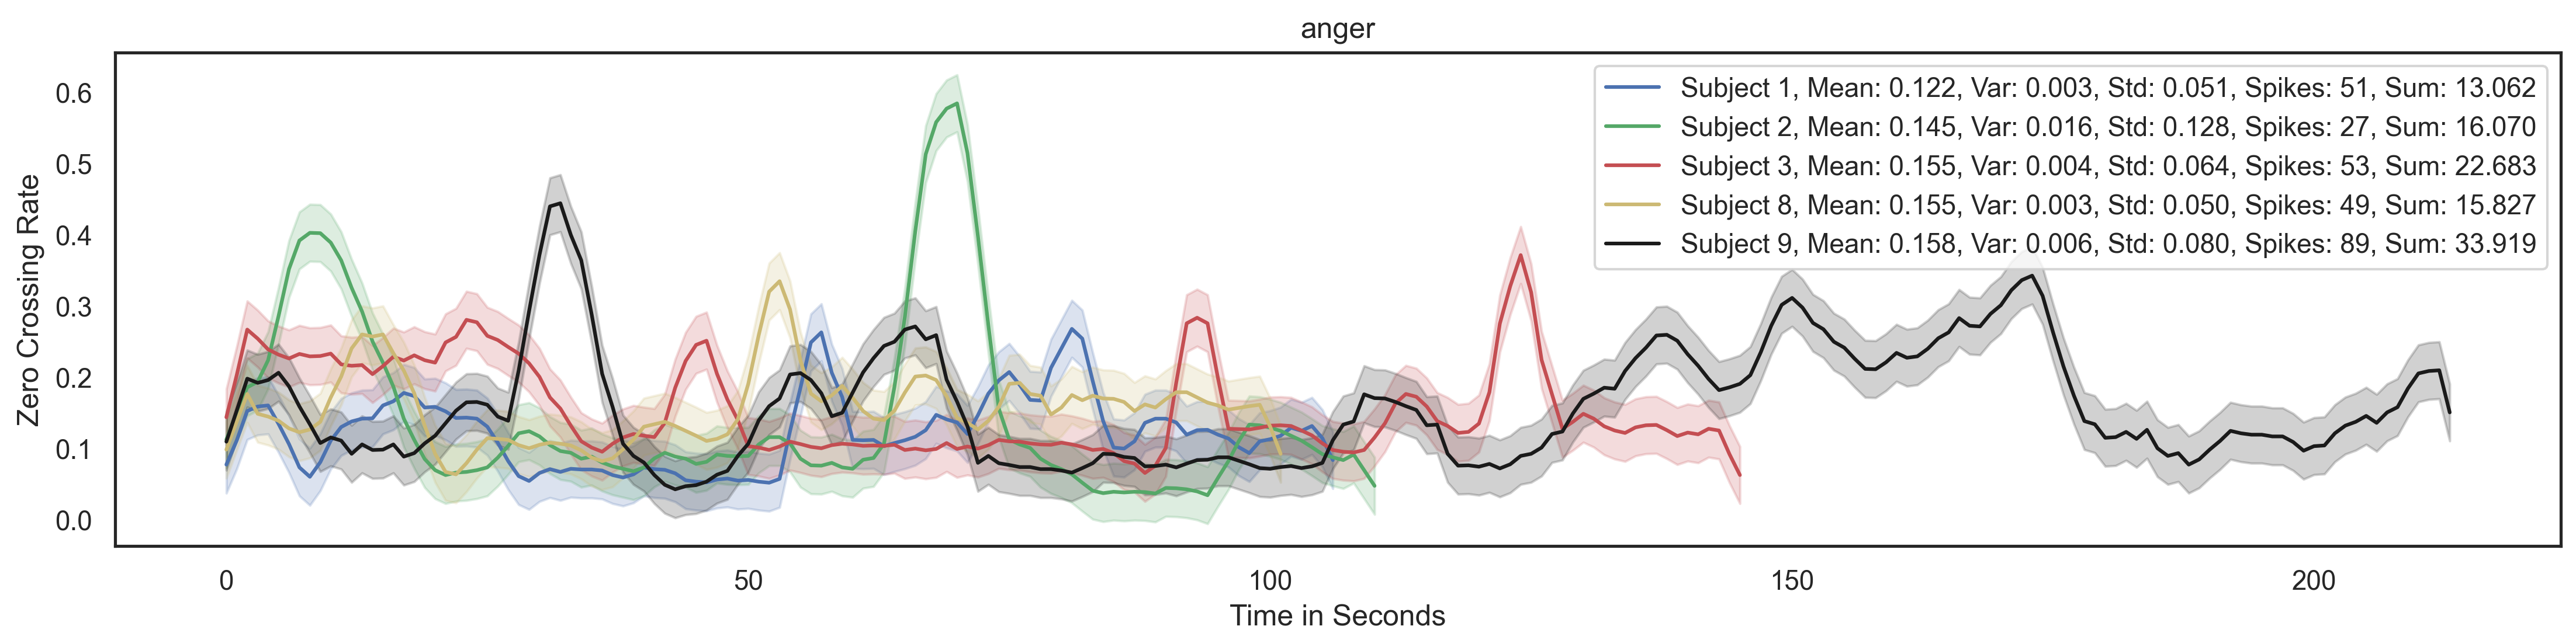
\includegraphics[width=1\linewidth]{figs/4_1_traditional/zcrAreaOnly1.png}
	\caption{Zero crossing rate wave plot with a surrounding area of five male subjects for the same utterance with the anger emotion.}
	\label{fig:zcrAreaOnly1}
\end{figure}

This same idea can also be used to determine whether a feature is favorable for creating a distinction between different emotions, which is naturally useful for the problem of classifying emotions. The conclusion can be drawn by observing the opposite of the previous example. If the areas around the zero crossing rate do not coincide too heavily, it is an indicator that the feature could be adequate for distinguishing different emotions.

Figure \ref{fig:zcrAreaSameSubj} displays six zero crossing rates of one subject saying the same sentence but expressing different emotions. As previously mentioned, since audio lengths are different, it is difficult to draw a direct and well-founded conclusion.

\begin{figure}[H]
	\centering
	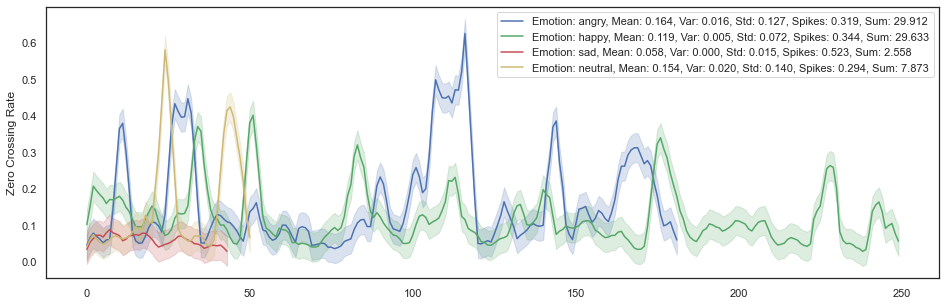
\includegraphics[width=.8\linewidth]{figs/4_1_traditional/zcr_male_same_subject.png}
	\caption{Zero crossing rate wave plots with a surrounding area of a single male subject and sentence for all different emotions.}
	\label{fig:zcrAreaSameSubj}
\end{figure}

Overall, this approach of surrounding wave plots with areas provided us valuable insight into the ability of a feature to describe and distinguish emotions, though it is a little limited by the varying lengths of audio segments.

\subsubsection{Variation Plots}

Another graph made was a variation plot, to perceive the differences in the features' values, across several audios for the same emotion. Figure \ref{fig:zcrMeanVar} shows an example of this type of plot for the mean zero crossing rate value across 50 speech utterances for all emotions.

\begin{figure}[H]
	\centering
	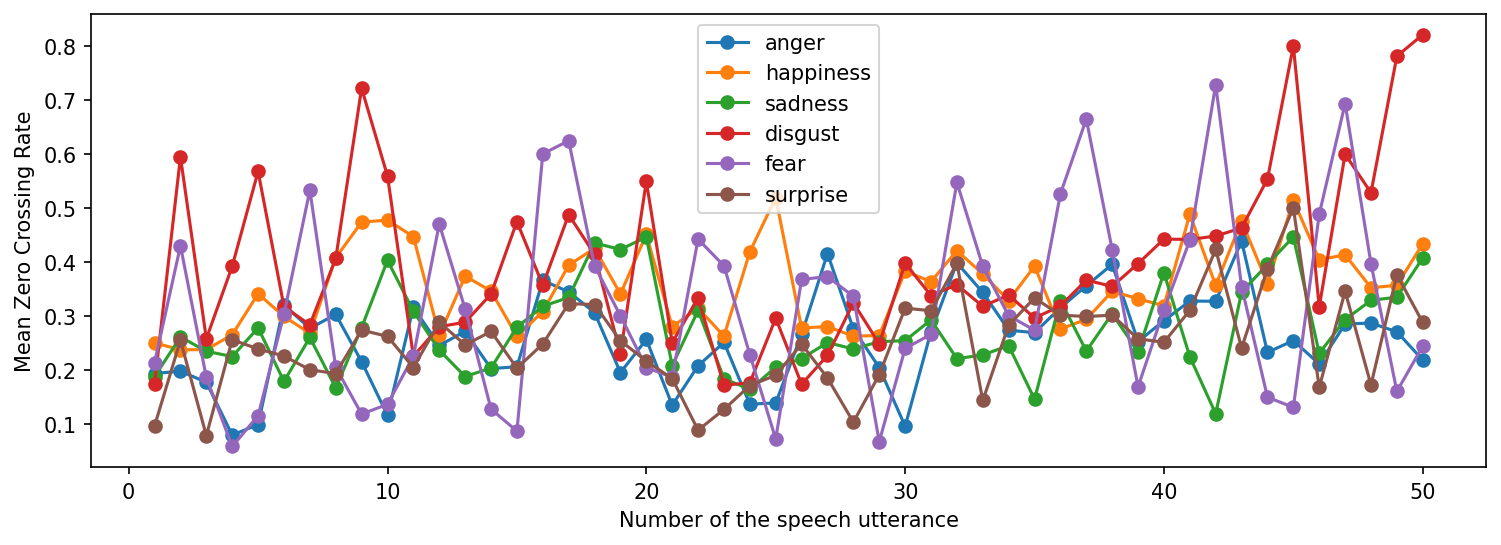
\includegraphics[width=\linewidth]{figs/4_1_traditional/meanZCRVar.png}
	\caption{Zero crossing rate mean values variation plot along 50 audios of speech utterances for all emotions}
	\label{fig:zcrMeanVar}
\end{figure}

A common observation for most extracted feature plots was that the values were not consistent across multiple audio segments for the same emotion. However, the number of audio segments used in this study was relatively low (only 50) to observe big variability changes, but increasing the number of audio segments would also make it more challenging to observe such variability through a simple visual inspection.

\subsubsection{Box Plots}

Finally, we employed box plots to visualize the distribution of the features on different subjects, as well as to compare the values for each emotion. An example of this type of plot is shown in Figure \ref{fig:zcrMeanBoxPlot}, which displays the mean zero crossing rate feature for all emotions and different subjects. 

\begin{figure}[H]
	\centering
	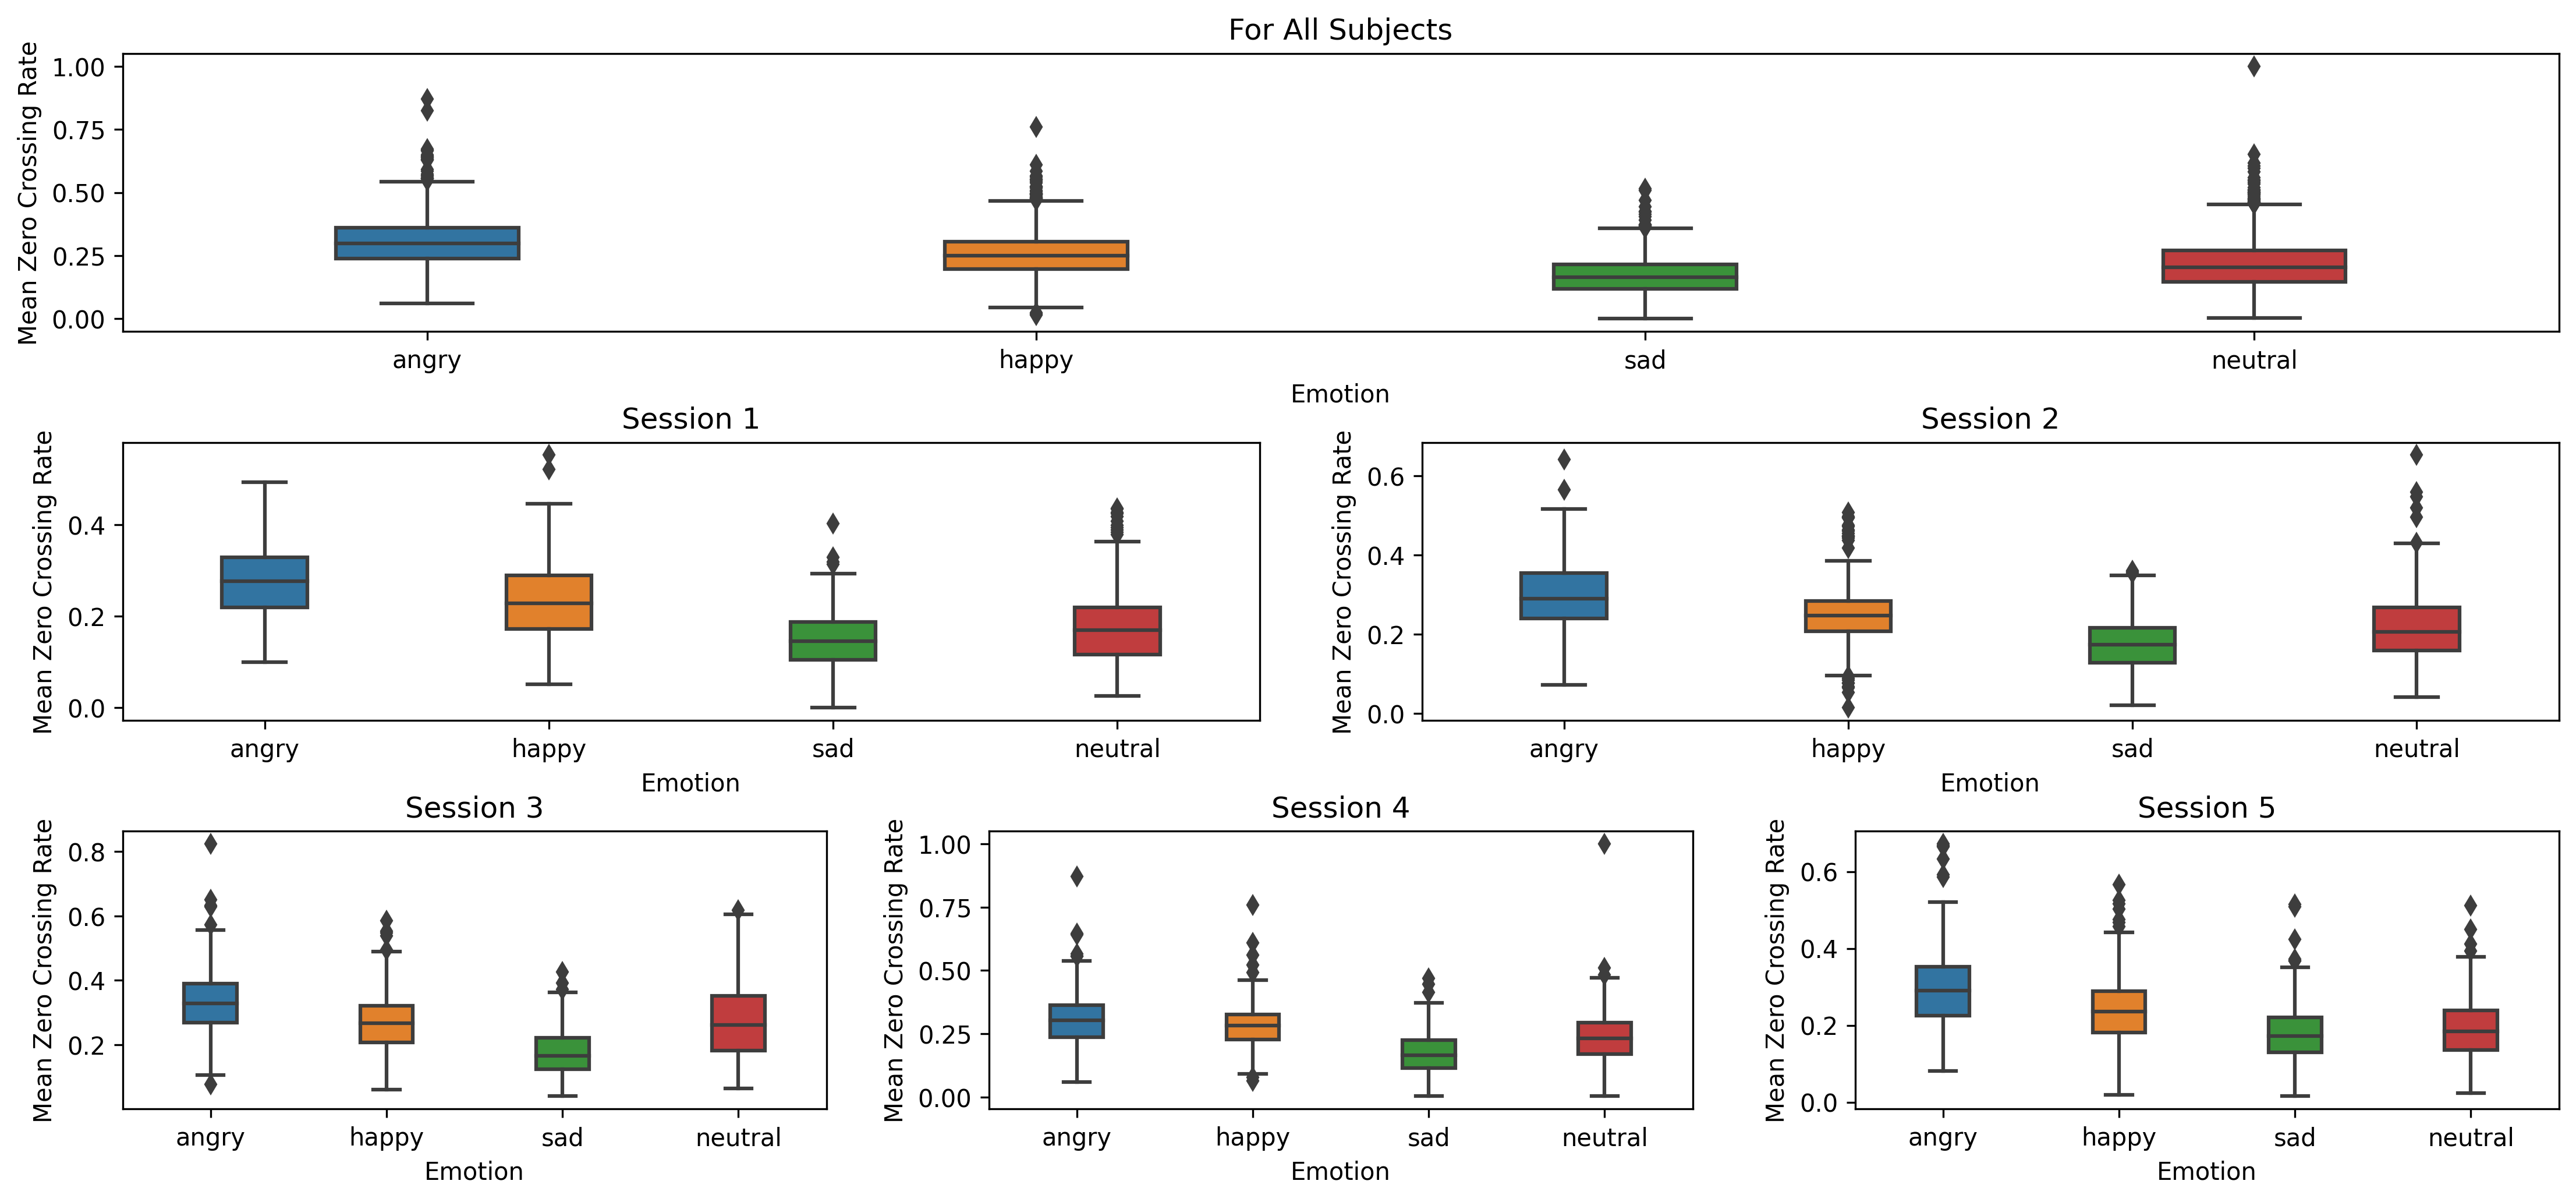
\includegraphics[width=\linewidth]{figs/4_1_traditional/mean_zcr_box_plot.png}
	\caption{Zero crossing rate mean values box plot for all emotions and different subjects}
	\label{fig:zcrMeanBoxPlot}
\end{figure}

The primary purpose of using these plots was to provide a simple and intuitive representation of each feature. By comparing the values across all subjects or a selected few, any noticeable differences in feature values for each emotion could be easily perceived.

\subsection{Feature Selection}

After the process of feature analysis, the next step in \ac{ser} development is feature selection. Feature selection is a technique to choose a subset of the original set of features that are most relevant for the given task. The process of feature selection is aimed to improve the accuracy of the model and reducing the problem's complexity by removing redundant or irrelevant features. 

The objective is to choose a smaller set of features that retain enough information for good classification performance while being computationally efficient. Hence, a smaller subset of features that can provide effective classification results is preferred over the larger set of features that may be computationally expensive and redundant.

\subsubsection{High Correlation Elimination}

Correlation among our extracted features is common since many of them use the same audio descriptor but with a different metric applied to them. Therefore, a correlation matrix for all 327 extracted features was calculated using the Pearson method, presented in figure \ref{allAudioFeat}.

A high correlation elimination was performed by selecting every pair of features with a Pearson correlation coefficient absolute value of 0.6 or above, then it was removed the feature with the highest average correlation value with all the other features. This process resulted in the elimination of 229 features, leaving 98 features for subsequent analysis. The correlation matrix after the feature selection process is presented in figure \ref{fig:highAudioFeat}.

\begin{figure}
	\centering
	\begin{subfigure}{.5\textwidth}
		\centering
		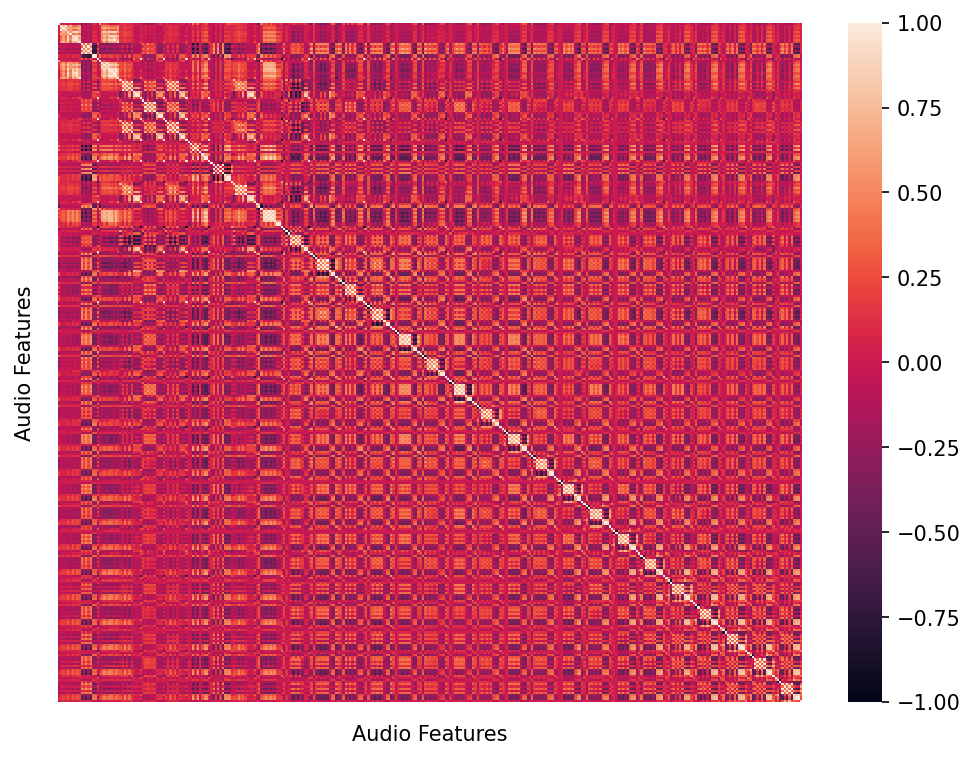
\includegraphics[width=\linewidth]{figs/4_1_traditional/allCorrMatrix.png}
		\caption{Correlation Matrix of all the Features.}
		\label{fig:allAudioFeat}
	\end{subfigure}%
	\begin{subfigure}{.5\textwidth}
		\centering
		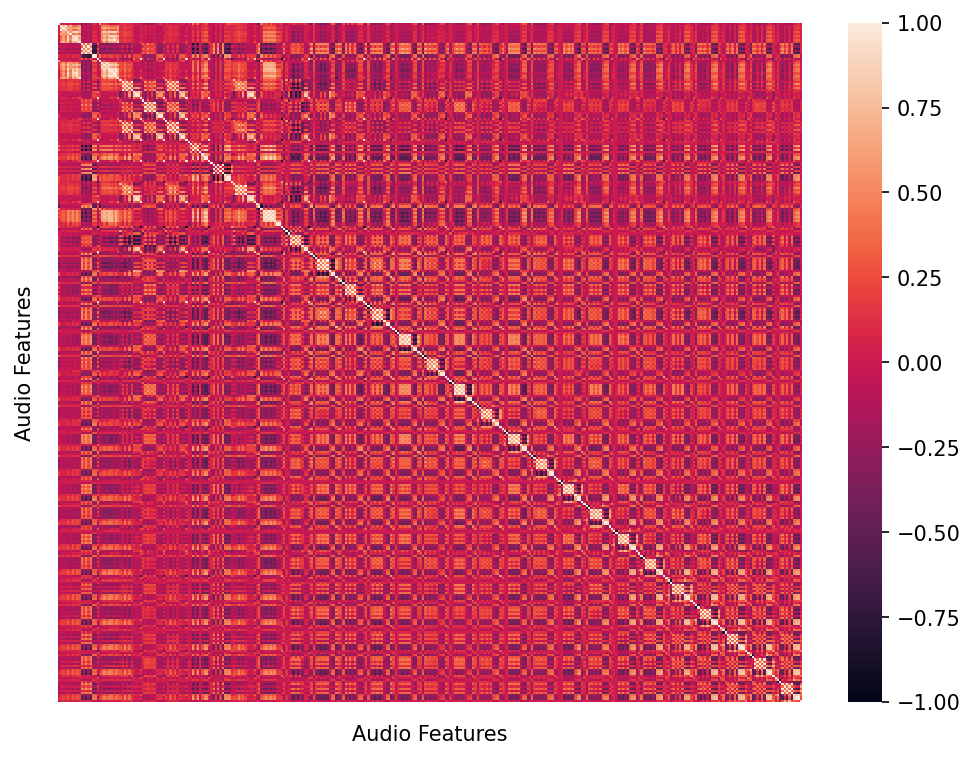
\includegraphics[width=\linewidth]{figs/4_1_traditional/highCorrMatrix.png}
		\caption{Correlation Matrix after High Correlation Elimination.}
		\label{fig:highAudioFeat}
	\end{subfigure}
	\caption{Audio Features' Pearson Correlation Matrices Before and After High Correlation Elimination.}
\end{figure}



\subsubsection{Selecting an Initial Classifier}

Along this process, it became necessary to choose a model to be used in computationally expensive feature selection methods. Consequently, several estimators were tested for their performance in classifying emotions.

To this end, we conducted 5-fold cross-validation and compared the mean and standard deviation accuracies of all folds, as well as the total execution time for various classifiers from the scikit-learn library \cite{pedregosa2011scikit}, using the features obtained after the previous process, as shown in Table \ref{tab:modelsPerformance}.

\begin{table}[H]
	\caption{Performance of various classifiers in 5-fold cross-validation using the features obtained after high correlation elimination.}
	\centering
	\label{tab:modelsPerformance}
	\begin{tabular}{lrrr}
		\toprule
		Classifiers &  Accuracy & Training Time (s) \\
		\midrule
		XGBoost                &        0.617$\pm$0.013  & 17.628 \\
		Random Forest          &        0.578$\pm$0.010  &  7.451 \\
		Ridge                  &        0.565$\pm$0.014  &  0.078 \\
		Extra Trees            &        0.561$\pm$0.005  &  1.831  \\
		AdaBoost               &        0.520$\pm$0.008  & 12.205  \\
		C-Support Vector       &        0.504$\pm$0.018  &  5.081 \\
		DecisionTree           &        0.450$\pm$0.022  &  1.886 \\
		Multi-layer Perceptron &        0.446$\pm$0.027  &  4.821 \\
		\bottomrule
	\end{tabular}
\end{table}

Based on the evaluation results, the Random Forest classifier was chosen for further analysis. This model exhibited the second best average accuracy across the 5 folds, however it was more than twice as fast the XGBoost that had highest average accuracy. Therefore, it was deemed suitable for performing computationally expensive feature selection methods.


\subsubsection{Backwards Selection}

In the pursuit of completing the feature selection process, a sequential feature selection with backward propagation was employed. This method involves performing a 5-fold cross-validation with the previously selected Random Forest classifier, using all features except one, and then removing one feature based on the lowest mean accuracy of the 5 folds. This iterative process continues until only one feature remains.

A method was then developed to select the furthest and highest accuracy. This method resembles the standard maximum, but it multiplies the maximum value by a threshold value of $0.99$, so that it can find close to the maximum values that have more features removed, creating a balance between accuracy and number of features. Figure \ref{fig:backProp1} displays the mean accuracies obtained at each step and the chosen furthest highest accuracy.

\begin{figure}[H]
	\centering
	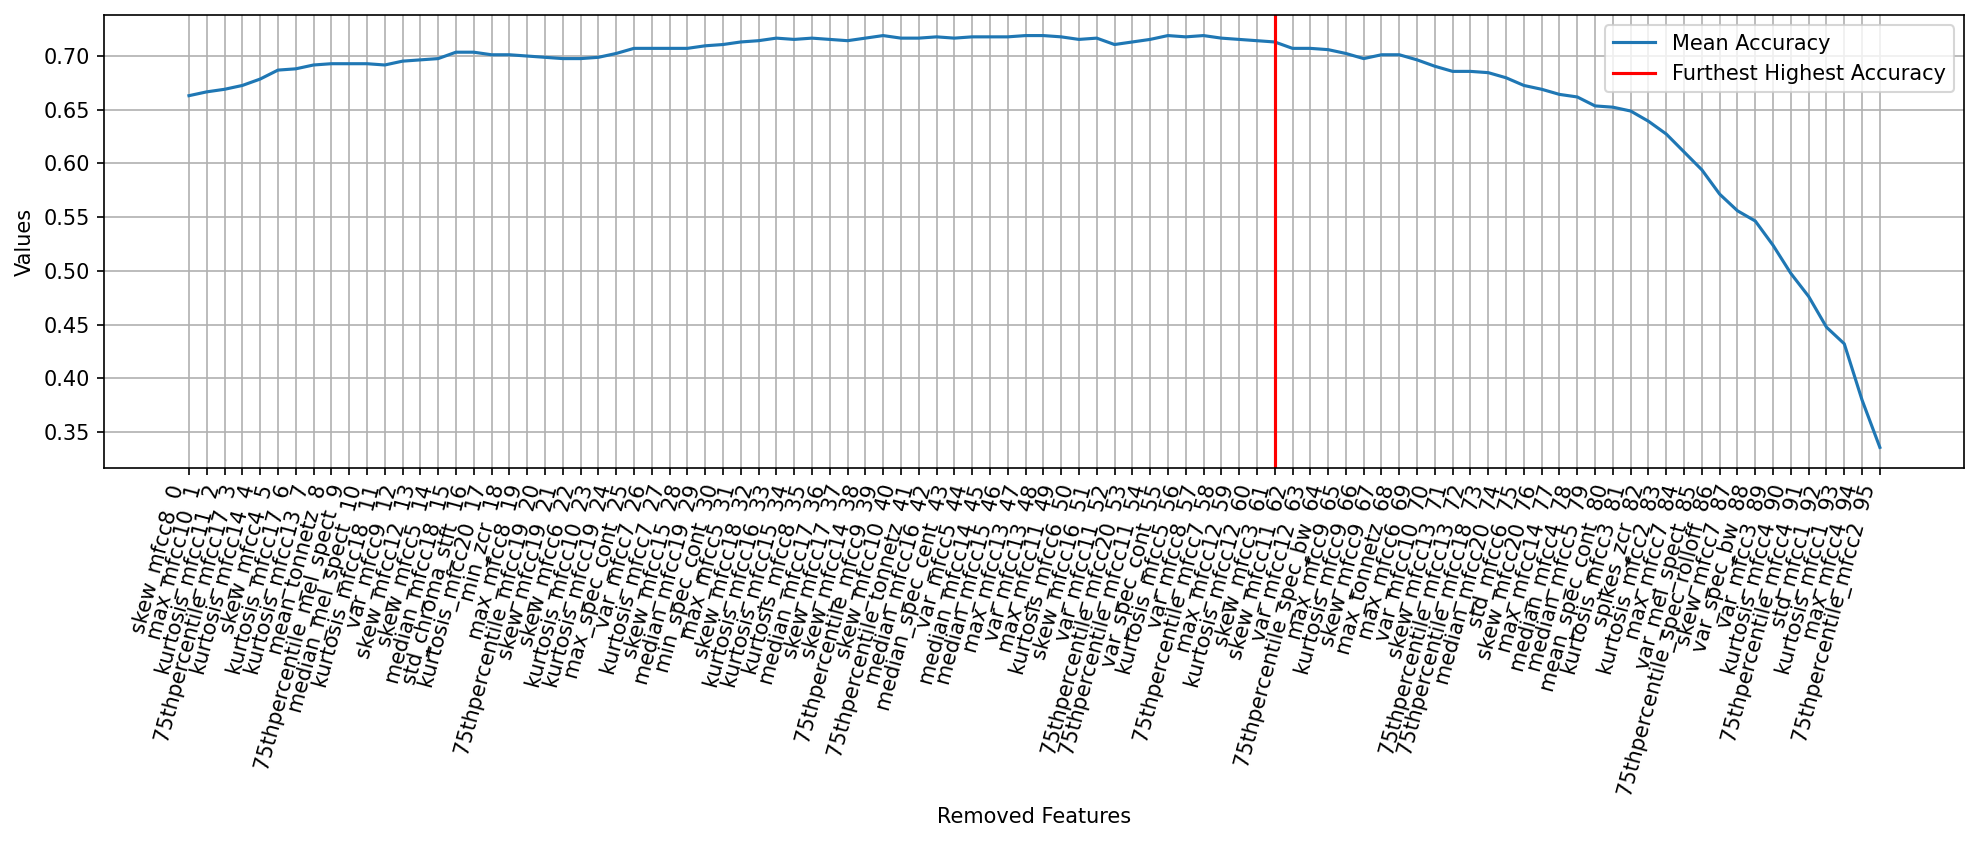
\includegraphics[width=1\linewidth]{figs/4_1_traditional/backProp1.png}
	\caption{Sequential Feature Selection with Backward Propagation using the Mean Accuracy as the Selection Method.}
	\label{fig:backProp1}
\end{figure}

This process led to the elimination of 65 features from the initial set of 98 obtained after the high correlation elimination, leaving a total of 33 features, as shown in Table \ref{tab:selectedFeat}.

\begin{table}[H]
	\caption{Selected features.}
	\centering
	\label{tab:selectedFeat}
	\resizebox{\textwidth}{!}{%
		\begin{tabular}{ll}
			\toprule
			Metric & Audio Features \\
			\midrule
			Spikes & Mel-Spectrogram, Chromagram, Zero Crossing Rate, MFCC-6, MFCC-16, MFCC-19 \\
			Mean & Spectral Bandwidth, MFCC-13, MFCC-15, MFCC-17, MFCC-19, MFCC-20 \\
			Maximum & Spectral Bandwidth, MFCC-5, MFCC-7, MFCC-10, MFCC-11 \\
			Variance & Mel-Spectrogram, MFCC-1, MFCC-3, MFCC-5, MFCC-8 \\
			Kurtosis & MFCC-12, MFCC-17, MFCC-18 \\
			25th Percentile & Chromagram, Root Mean Square \\
			75th Percentile & MFCC-7, MFCC-11 \\
			Sum & MFCC-10, MFCC-12 \\
			Median & MFCC-5 \\
			Min & Zero Crossing Rate \\
			\bottomrule
		\end{tabular}
	}
\end{table}



\subsubsection{Feature Selection Evaluation}

To assess the feature selection quality on the development dataset, we trained and evaluated the predictions of a Random Forest Classifier model with different sets of features, using accuracy as the evaluation metrics. The results are presented in Table \ref{tab:acc}. Additionally, we plotted the confusion matrix of the predictions, which can be found in Appendix \ref{confusionMatrices}.

\begin{table}[H]
	\caption{Evaluation Metrics of Random Forest Predictions Using Different Sets of Features and 5-Fold Cross Validation.}
	\centering
	\label{tab:acc}
	\begin{tabular}{lrrr}
		\toprule
		Feature Selection Method & N.º of Features & Accuracy & Training Time (s)\\
		\midrule
		None & 327 & 59.14$\pm$0.68 & 15.34 \\
		High Correlation Elimination & 98 & 57.87$\pm$1.07 & 7.89 \\
		\begin{tabular}{@{}l@{}}High Correlation Elimination \&\\Backward selection\end{tabular} & 33 & 59.12$\pm$1.05 & 4.29\\
		\bottomrule
	\end{tabular}
\end{table}

The results of the feature selection techniques have shown that while there may be a small loss of accuracy between the initial set of extracted features and the set obtained after the high correlation elimination, the model can achieve comparable accuracy while using only around 70\% of the original set. Moreover, applying backward selection to the remaining 98 features yields optimal results by maintaining the accuracy and reducing the original feature set by approximately 90\%.

By using these feature selection techniques, we managed to remove redundant and irrelevant features, which also decreases the models' complexity and size, providing several practical benefits for its implementation and interpretation.


\subsection{Classifiers Evaluation and Selection}

\subsubsection{Evaluation Strategy}
TODO: explain each metric maybe

Evaluating a model is an essential step, since a wrongful evaluation may lead to deception in terms of the results obtained. It should be uniform for every model, and, it should be as meaningful as possible to the classification objective.

As mentioned previously, for this part and the subsequent parts of the \ac{ser} development, the second dataset \ac{iemo} is the one under use.

For the reasons above, it was decided to utilize 5-fold cross-validation, and, in terms of metrics, we decided to calculate 5 folds averages accuracy, macro-f1 score, precision, recall, and \ac{mcc}. A confusion matrix of the predicted and real labels was also plotted, since it provides helpful insights, not only into the errors being made by the classifier but also, the types of errors occurring.

These were also the most recurred methods in state-of-the-art research, which provides more fairness to model comparisons.

\subsubsection{Classifiers Exploration}

An Automatic Machine Learning technique, namely Auto-SKLearn ensemble model \cite{feurerneurips15a}, was employed to search for the best models and ensembles by exploring a vast space of possible algorithms and hyperparameters using a meta-learning approach.

After training the Auto-SKLearn model, the most influential classifiers of the ensemble were identified, resulting in an ensemble with 9 classifiers, including Random Forests with different hyperparameters, Linear Discriminant Analysis, Histogram-Based Gradient Boosting, Multilayer Perceptron, and Linear Passive Aggressive. Each model present in the ensemble was then tested and explored.

Next, a simple Convolutional Neural Network was tested, and another AutoML technique, AutoKeras \cite{jin2019auto}, was applied to create an optimized deep-learning model.

\subsubsection{Results and Conclusions}

The results obtained from the tested models were compiled and exhibited in Table \ref{tab:models}. The highest-ranked Random Forest from the Auto-SKLearn ensemble model achieved the best results, leading to its selection as the base estimator of an AdaBoost classifier, improving slightly the overall Random Forest results.

\begin{table}[H]
	\centering
	\caption{Tested Classification Models 5-Fold Cross-Validation Performance on \ac{iemo}.}
	\label{tab:models}
	\begin{tabular}{lrrrrrr}
		\toprule
		Model & Accuracy & Macro F1 & Precision & Recall & \ac{mcc} & Training Time \\
		\midrule
		
		AdaBoost & 60.04$\pm$0.95 & 60.76 & 61.29 & 60.59 & 0.459 & 8.45  \\
		
		Random Forest & 59.77$\pm$0.72 & 60.43 & 60.97 & 60.30 & 0.456 & 50.62 \\
		
		Histogram Gradient Boosting & 59.25$\pm$1.53 & 59.80 & 60.34 & 59.47 & 0.450 & 133.31  \\
		
		XGBoost & 58.09$\pm$1.34 & 58.74 & 59.30 & 58.44 & 0.431 & 7.37 \\
				
		Balanced Random Forest & 56.92$\pm$0.83 & 57.31 & 56.90 & 59.84 & 0.432 & 11.29  \\
		
		Ridge & 53.28$\pm$0.98 & 54.14 & 53.94 & 54.44 & 0.369 & 0.02 \\
				
		Linear Discriminant Analysis & 54.04$\pm$1.38 & 55.06 & 55.01 & 55.23 & 0.379 & 0.06 \\
		
		\ac{lstm} & 51.0$\pm$0.54 & 51.42 & 51.35 & 51.87 & 0.339 & 775.95 \\
		
		\ac{cnn} & 50.41$\pm$0.95 & 51.25 & 51.61 & 52.69 & 0.340 & 340.74  \\
		
		\bottomrule
	\end{tabular}
\end{table}



\begin{table}[H]
	\centering
	\caption{\ac{sota} Traditional Classification Models Performance on \ac{iemo}.}
	\label{tab:modelssoa}
	\begin{tabular}{lcr}
		\toprule
		Model                        &   Input &   Accuracy \\
		\midrule
		
		Dilated Residual Network \cite{Li_2019}	& Audio Features & 67.4 \\
		
		\ac{rnn} W/ Attention \cite{Lu_2020} & Audio and Text Features & 72.6 \\
		
		Deep \ac{cnn} \cite{Issa_2020} & 193 Audio Features & 64.30 \\
		
		\bottomrule
	\end{tabular}
\end{table}


The application of data preprocessing techniques to clean the audio data was performed to handle different technical settings. However, in some cases, noise may be part of the signal of interest, and removing it may cause the algorithm to misinterpret the signal.

The state-of-the-art results presented in Table \ref{tab:modelssoa} are not directly comparable, as authors use different data and evaluation methodologies. Additionally, some authors do not consider the emotion of excitement as happiness or perform different validation methods such as 10-fold cross-validation.

Upon analyzing the explored classifiers results, AdaBoost with Random Forest as the base estimator is the best candidate, reaching an average accuracy of 60.04\% while utilizing only 33 audio features which makes it a model that is relatively simple, fast to train and make predictions, while also being generalized to different datasets due to the preprocessing techniques applied. The Python code for the model was implemented using the SK-Learn library, version 1.2.1, and is presented on the following  Code Snippet \ref{tra:code}.

\begin{listing}[H]
	\begin{minted}{python}
AdaBoostClassifier(estimator=RandomForestClassifier(n_estimators=512))
	\end{minted}
	\caption{Python code for the selected AdaBoost classifier using the traditional-based \ac{ser} approach.}
	\label{tra:code}
\end{listing}